              
% ****** Start of file apssamp.tex ******
%
%   This file is part of the APS files in the REVTeX 4.1 distribution.
%   Version 4.1r of REVTeX, August 2010
%
%   Copyright (c) 2009, 2010 The American Physical Society.
%
%   See the REVTeX 4 README file for restrictions and more information.
%
% TeX'ing this file requires that you have AMS-LaTeX 2.0 installed
% as well as the rest of the prerequisites for REVTeX 4.1
%
% See the REVTeX 4 README file
% It also requires running BibTeX. The commands are as follows:
%
%  1)  latex apssamp.tex
%  2)  bibtex apssamp
%  3)  latex apssamp.tex
%  4)  latex apssamp.tex
%
\documentclass[%
 reprint,
%superscriptaddress,
%groupedaddress,
%unsortedaddress,
%runinaddress,
%frontmatterverbose, 
%preprint,
%showpacs,preprintnumbers,
%nofootinbib,
%nobibnotes,
%bibnotes,
 amsmath,amssymb,
 aps,
%pra,
%prb,
%rmp,
%prstab,
%prstper,
%floatfix,
]{revtex4-1}

\usepackage{graphicx}% Include figure files
\usepackage{dcolumn}% Align table columns on decimal point
\usepackage{bm}% bold math
\usepackage{hyperref}% add hypertext capabilities
%\usepackage[mathlines]{lineno}% Enable numbering of text and display math
%\linenumbers\relax % Commence numbering lines

%\usepackage[showframe,%Uncomment any one of the following lines to test 
%%scale=0.7, marginratio={1:1, 2:3}, ignoreall,% default settings
%%text={7in,10in},centering,
%%margin=1.5in,
%%total={6.5in,8.75in}, top=1.2in, left=0.9in, includefoot,
%%height=10in,a5paper,hmargin={3cm,0.8in},
%]{geometry}
\bibliographystyle{plain}

%\graphicspath{{C:\Users\Nick\Documents\GitHub\FYS2150\lab1}}

\begin{document}

%\preprint{APS/123-QED}

\title{FYS2150 \\
Lab Report: Time and Frequency}% Force line breaks with \\

\author{Nicholas Karlsen}
% \email{nichoka@student.matnat.uio.no}

\date{\today}% It is always \today, today,
             %  but any date may be explicitly specified

\begin{abstract}
The goal for this lab was measuring time, and comparing three methods of doing so, of varying degrees of "sophistication"; an hourglass, a stopwatch and a photodiode.
\end{abstract}

\maketitle

%\tableofcontents

\section{\label{sec:intro}Introduction}
	The lab spanned 6 hours and consisted of measuring the period of a pendulum using three different methods of measurement; an hourglass, a stopwatch and a photodiode connected to a computer. The experiments were performed by myself, and my lab partner Lars K. Skaarseth.
	Before anything else, it is worth to note that the first experiment can largely be disregarded due to an error on our part, more on this in section \ref{subsect:exp_stopwatch}.

\section{Theory}
	The theory used in this lab report is almost entirely summed up by the following equations;
	\begin{equation}
        \label{eqn:period}
		T = 2\pi \sqrt{\frac{L}{g}}
	\end{equation}
	Where $T$ denotes the period a swinging pendulum, $L$ the length of the wire by which the pendulum is suspended and $g$ the downward acceleration on the pendulum due to gravity.
	\begin{equation}
		\vec R = \frac{1}{M} \sum_i m_i \vec r_i
	\end{equation}
	Where $\vec R$ denotes the position of the center of mass of a body of mass $M$ consisting of several smaller bodies of mass $m_i$ with individual center of mass at $r_i$.

	Further detail can be found in "Elementary Mechanics Using Python" \cite{elempy}, or most other books covering introductory mechanics.

\section{\label{section:experimentalproced}Experimental Procedure}
    
    We connected an aluminium cyllinder to a block of aluminium secured to a desk with a (i believe nylon?) string as shown in Fig. \ref{fig:pendulum1}. For the purposes of this experiment the string is asumed to be inextensible. 

    The string was turned on the Outer side of the screws on the top block, and the inner at the bottom so that the string would form a "V" shape, or positive angle. This was done in an attempt to limit the sideways motion of the block as much as possible, so that more of its kinetic energy would be restricted to the forward/backward motion (from the perspective of Fig. \ref{fig:pendulum1}), which is the motion being measured in these experiments.

    The length of the string, and later, the dimensions of the pendulum (As shown in Fig. \ref{fig:pendulum1}) were measured using a Hultafors meter-rule with an uncertainty of $\pm 1mm$ as well as a small uncertainty due to thermal expansion. Since we did not record the temperature in the room, i will assume standard temperature and pressure, thus negating the need to account for thermal expansion.

    \begin{figure}
        \center
        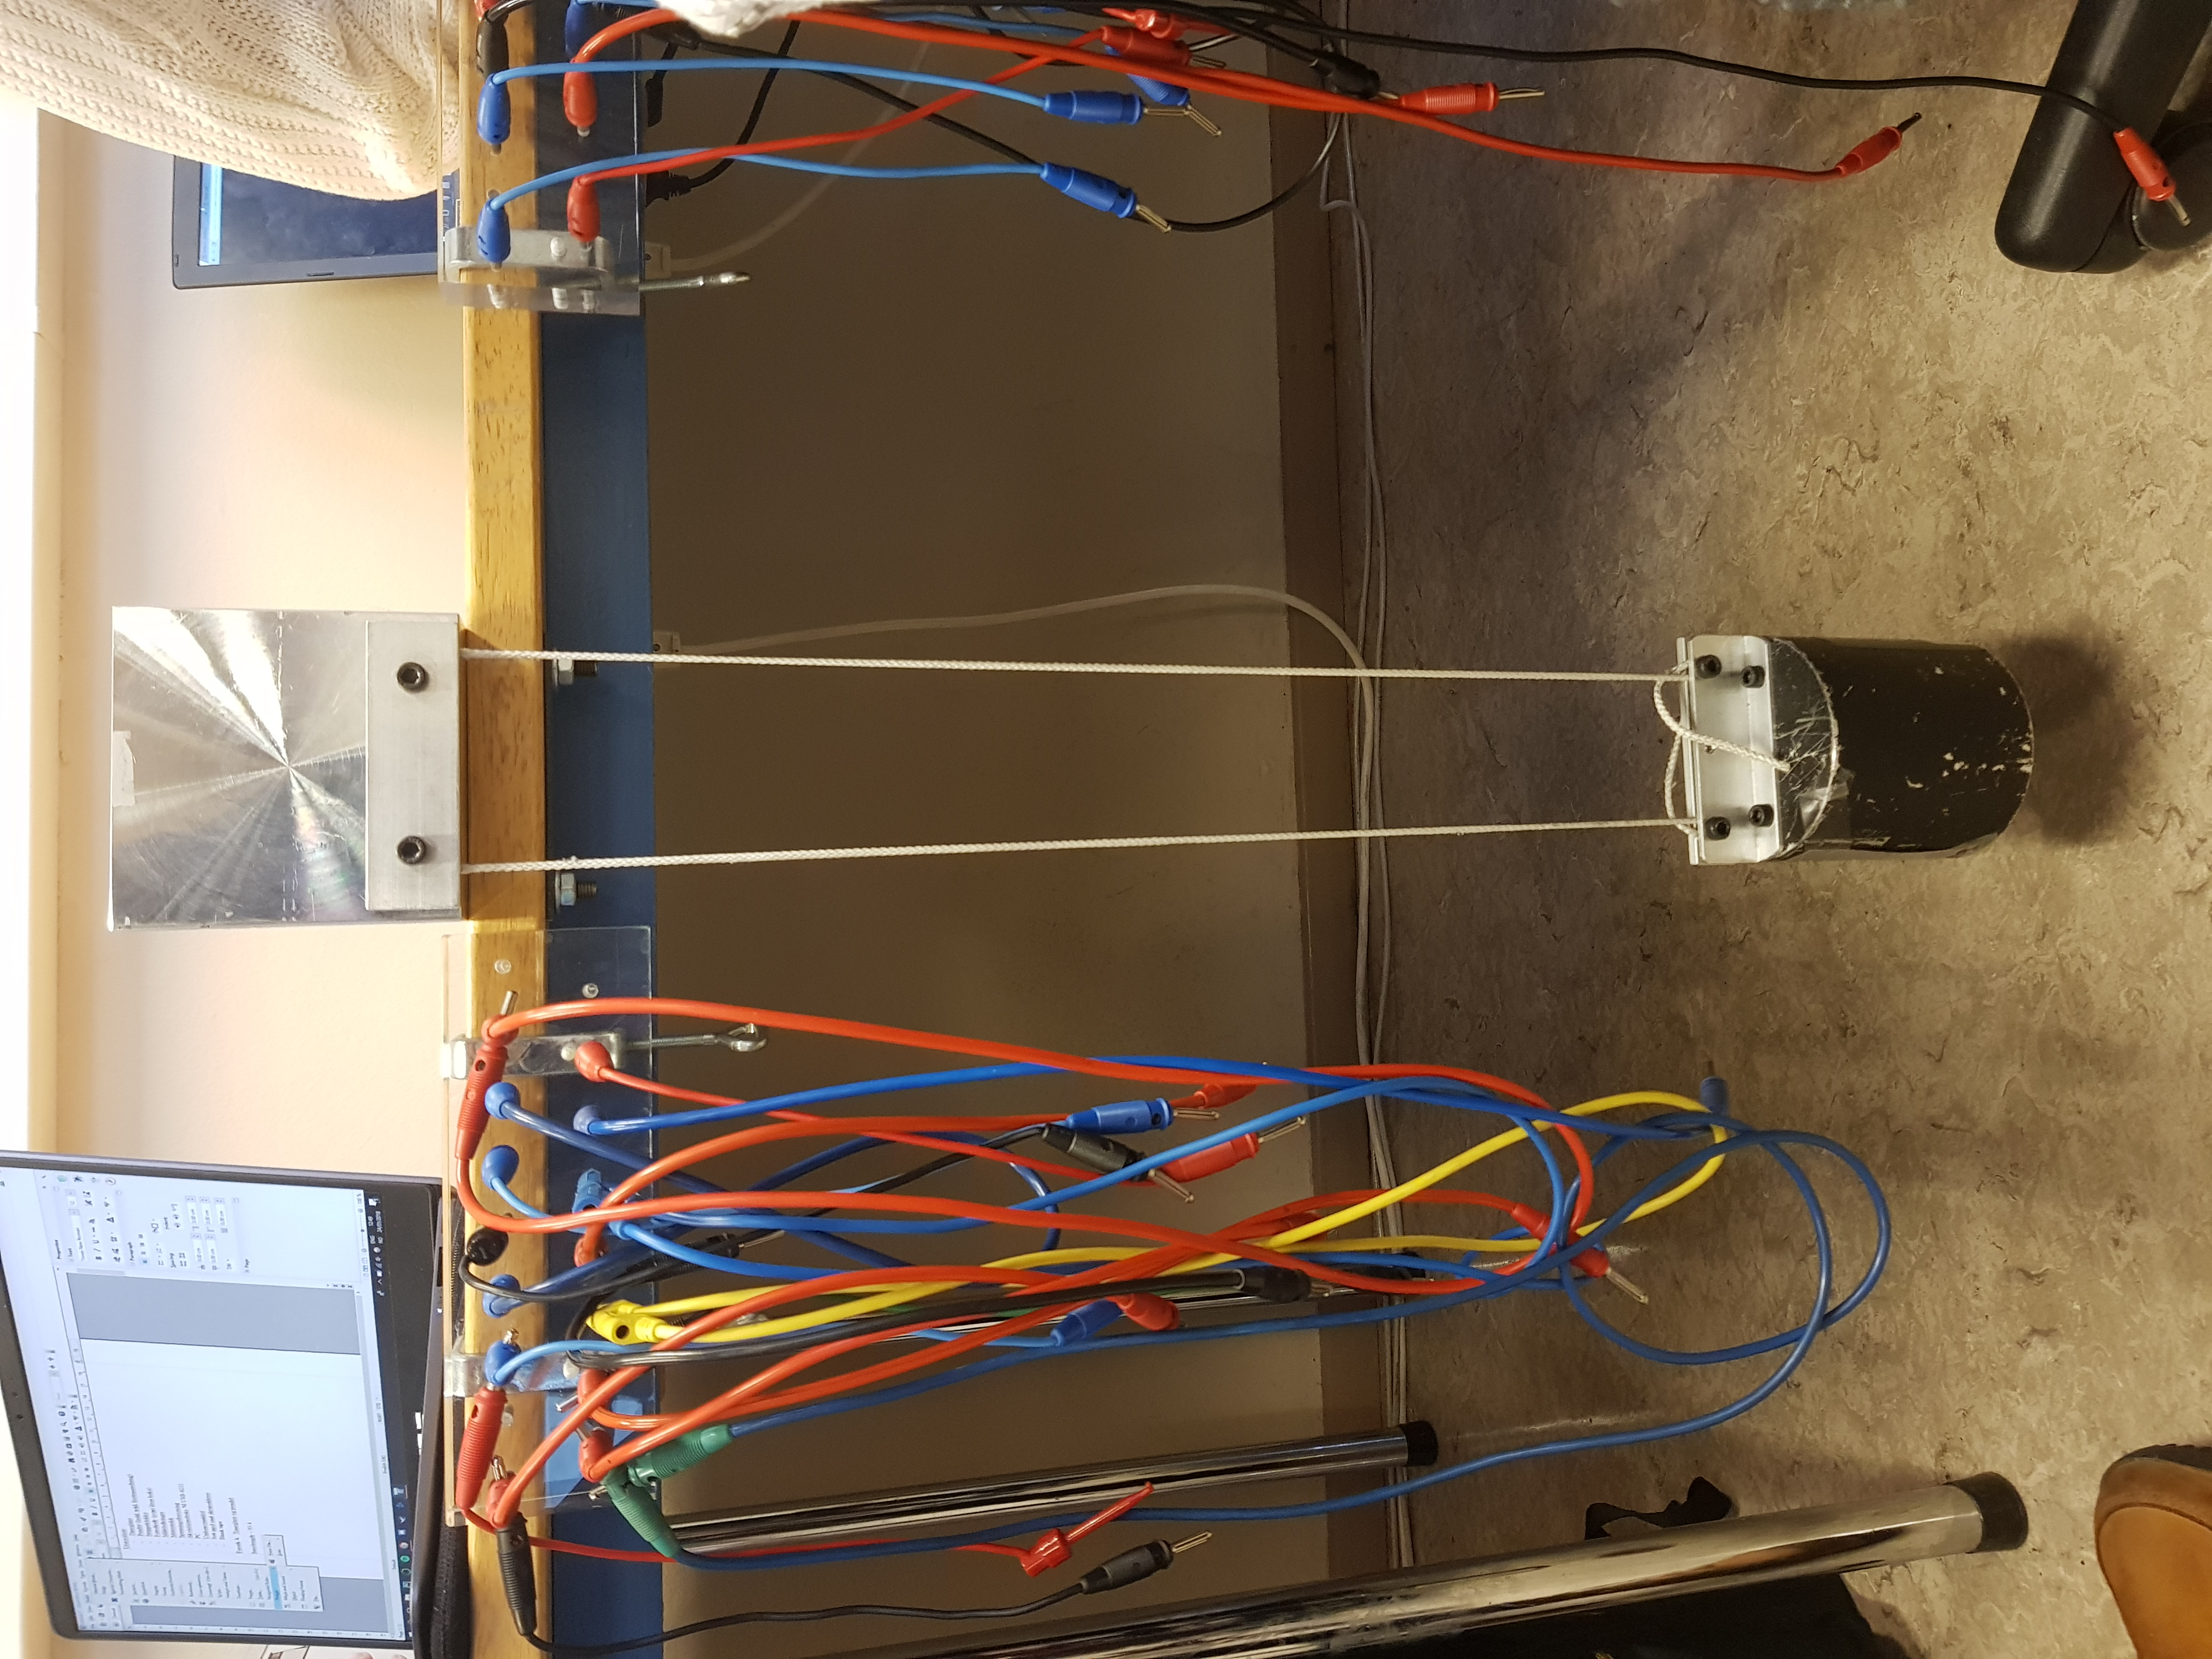
\includegraphics[scale=0.06, angle=270]{experiment1.jpg}
        \caption{A photograph showing how the pendulum was set up}
        \label{fig:pendulum1}
    \end{figure}

    \subsection{\label{subsec:exp_hourglass}Hourglass}
        In this this initial part of the experiment, we wanted to measure the number of swings made by the pendulum for the duration of an hourglass with an unknown duration. After having released the pendulum, we let it swing for one period before starting the hourglass, then both i and my lab partner then counted the number of swings separately in an attempt to minimize the chance human error when counting. Since we only counted complete swings, the measured value has an uncertainty of $\pm 1T$. The hourglass was also kept still on a table for its complete duration.
    
    \subsection{\label{subsect:exp_stopwatch}Stopwatch}
        This part is mostly similar to the last one, the only difference being the method of measuring the period. This time we used a stopwatch (Cielo 100MT, uncertainty of $\pm 0.01s$) to record the time. In order to minimize human error, we opted to only measure the time every 10th swing and again, both of us counted the swings individually ensuring we would not record the time at the wrong number of swings. We used the lap function of the stop watch to save the time taken for every 10th swing as well as the total running time for the 100 swings that we recorded.

        A rather signifficant source of error in this experiment comes from the reaction time, and to some extent the judgement of the person who is recording the time (he had to judge when the pendulum was at its apex).


	\subsection{\label{subsect:exp_photodiode}Photodiode}

        \begin{figure}
            \center
            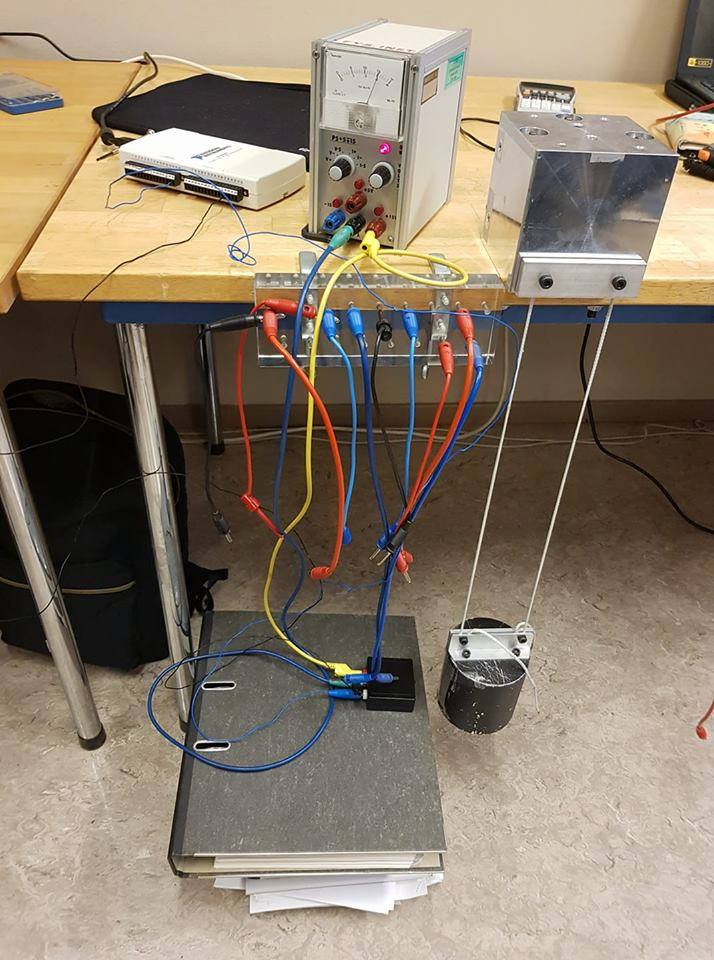
\includegraphics[scale=0.3]{experiment3.jpg}
            \caption{A photograph showing how the photodiode was set up and connected to the data aquisition box (NI USB-6211) for experiment no. 3 (Section \ref{subsect:exp_photodiode})}
            \label{fig:pendulum3}
        \end{figure}

        In this part, we made our measurements electronically using a photodiode connected to a computer with matlab via a data aquisition box (NI USB-6211). A photodiode sends out IR light, when this light is not reflected back to an IR sensitive reciever, the photodiode emits a constant 5V . When the IR light is reflected back to it, it instead emits 0V. For this reason, we had to attach a reflective material to the block of aluminium. We opted for some aluminium foil.
        Once everything was properly connected (see Fig. \ref{fig:pendulum3}) we ran a matlab script \href{http://www.uio.no/studier/emner/matnat/fys/FYS2150/v18/kursmateriell/tid-og-frekvens/svingeperiode.m}{\textbf{svingeperiode.m}} to record the data and started the pendulum as previously. We repeated this 4 times with different settings and conditions.



\section{\label{sect:results}Results}
	\subsection{Pendulum \& Hourglass}

	\begin{table} % Pendulum and hourglass
        \center
        \caption{Measurements with Hourglass}
        \label{tab:hourglass}
        \begin{tabular}{| l | l |}
            \hline
            Recording no. & Number of oscilations $(\pm 1)$\\ \hline
            1 & 116 \\ \hline
            2 & 121 \\ \hline
            3 & 128 \\ \hline
        \end{tabular}
	\end{table}

	\subsection{Pendulum \& Stopwatch}

	\begin{table} % Pendulum and stopwatch
        \center
        \caption{Measurements with Stopwatch}
        \label{tab:stopwatch}
	    \begin{tabular}{| p{1.5cm} | p{2cm} | p{2cm} |}
		    \hline
		    Number of periods & Time [sec] ($\pm 0.01$) & Total time [min:sec] ($\pm 0.01$)\\ \hline
		    10 & 14.14 & 14.14 \\ \hline
		    20 & 14.31 & 28.53 \\ \hline
		    30 & 14.32 & 42.85 \\ \hline
		    40 & 14.40 & 57.25 \\ \hline
		    50 & 14.29 & 1:11.54 \\ \hline
		    60 & 14.39 & 1:25.93 \\ \hline
		    70 & 14.29 & 1:40.72 \\ \hline
		    80 & 14.34 & 1:54.46 \\ \hline
		    90 & 14.20 & 2:08.76 \\ \hline
		    100 & 14.52 & 2:23.28 \\ \hline
        \end{tabular}
    \end{table}
    
    \subsection{Pendulum \& Photodiode}

    \begin{table} % Pendulum and stopwatch
        \caption{Measurements with photodiode}
        \label{tab:photodiode}
        \begin{tabular}{| p{1.7cm} | p{1.5cm} | p{1.5cm} | p{1.5cm} | p{1.5cm} | p{1.5cm} |}
            \hline
            Experiment no. & Standard deviation of mean period & Mean period & Position of diode & Total measured time [s] & Measuring frequency [KHz] \\ \hline
            1 & 5.6540e-4 & 1.4421 & Bottom & 120 & 25 \\ \hline
            2 & 8.8552e-4 & 1.4502 & Bottom & 120 & 200 \\ \hline
            3 & 0.0483 & 1.5816 & top & 120 & 25 \\ \hline
            4 & 0.0026 & 1.4922 & Bottom & 120 & 25 \\ \hline
        \end{tabular}
    \end{table}
    
    \begin{figure}[h!]
    	\center
    	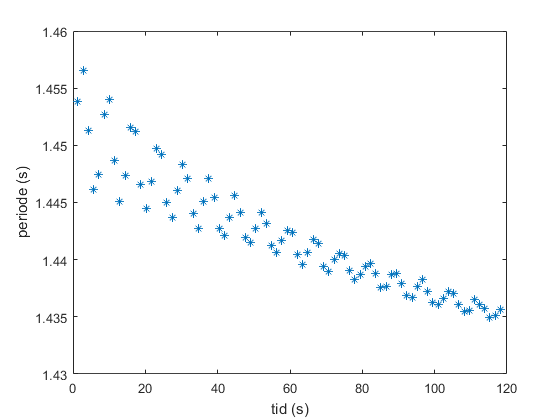
\includegraphics[scale=0.6]{forsok1fig1}
    	\caption{Data from Experiment no. 1 using the photodiode
    	\footnote{Due to bad planning on my part, this figure, and the following all lack figure titles.
    	}}
    \end{figure}

    \begin{figure}[h!]
    	\center
    	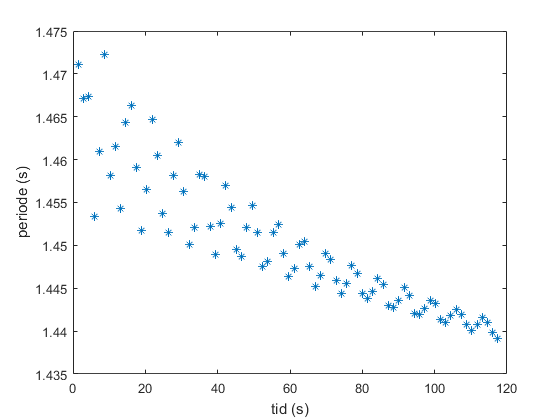
\includegraphics[scale=0.6]{forsok2fig1}
    	\caption{Data from Experiment no. 2 using the photodiode}
    \end{figure}

    \begin{figure}[h!]
    	\center
    	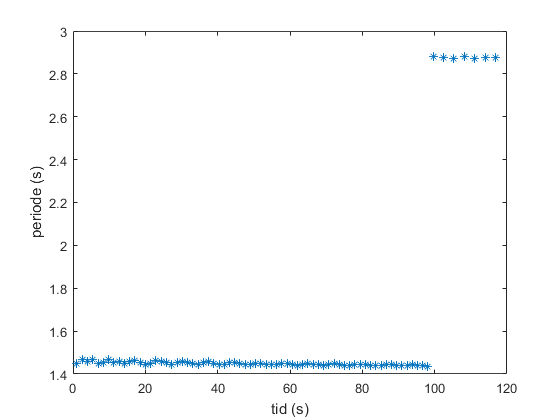
\includegraphics[scale=0.6]{forsok3fig1}
    	\caption{Data from Experiment no. 3 using the photodiode}
    \end{figure}

    \begin{figure}[h!]
    	\center
    	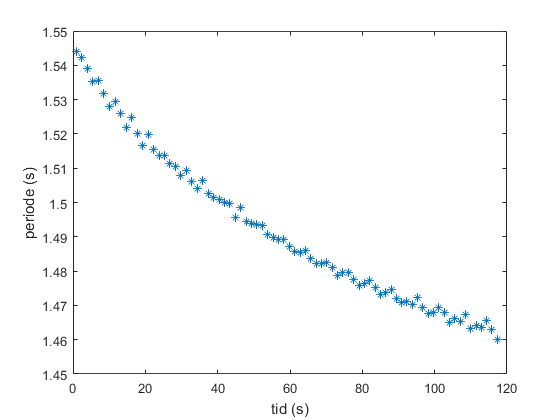
\includegraphics[scale=0.6]{forsok4fig1}
    	\caption{Data from Experiment no. 4 using the photodiode}
    \end{figure}


  	

\section{Discussion}
 
\section{Conclusion}
	

\bibliography{rapport1_ref}

\end{document}
%
% ****** End of file apssamp.tex ******
              